\subsection{a}
\begin{figure}[h]
	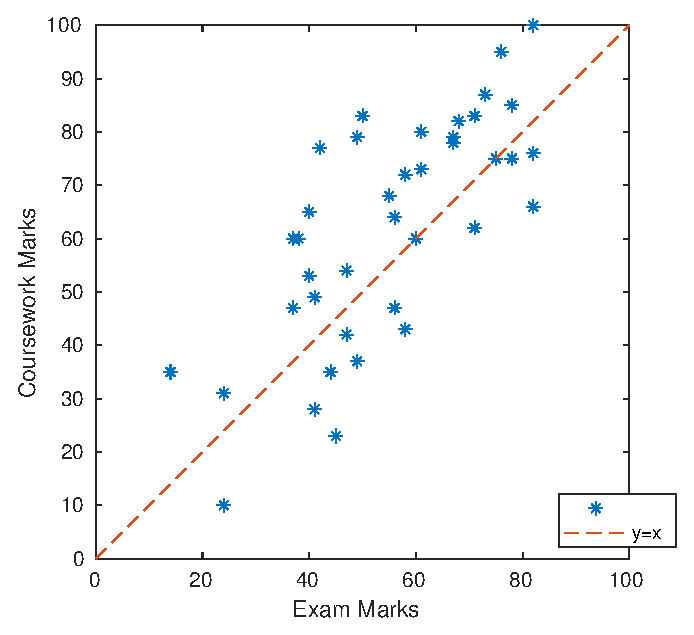
\includegraphics[scale=0.8, center]{./eps/topic1_a.eps}
    \caption{Coursework marks plotted against exam marks. Note the orange dashed line of symmetry}
    \label{fig:Topic1-a}
\end{figure}
In Figure \ref{fig:Topic1-a} the line of symmetry, $x=y$, was plotted.
Because the data are reasonably spread around the line of symmetry, there is evidence for some proportionality between the two data sets.
\lstinputlisting[caption={Topic 1. Question a. Note all code per topic belongs to same file}]{"./files/topic 1/a.m"}

\pagebreak

\subsection{b}
\begin{figure}[h]
	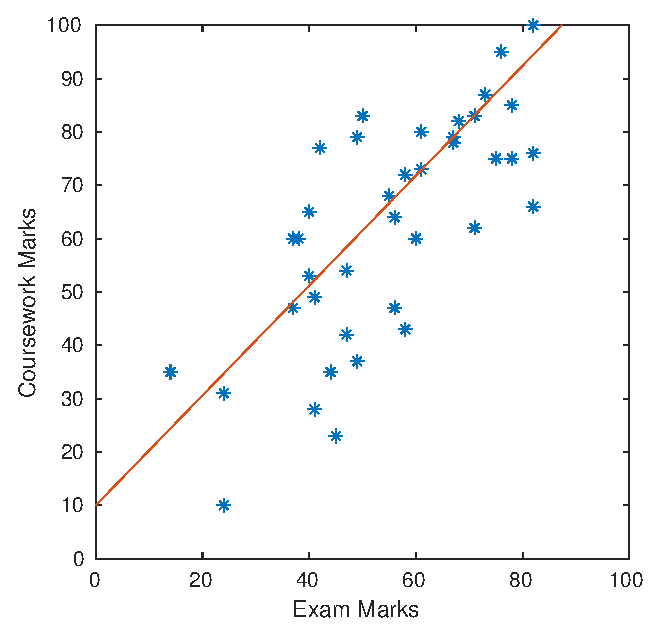
\includegraphics[scale=0.8, center]{./eps/topic1_b.eps}
	\caption{Coursework marks plotted against exam marks. Line of best fit estimated by eye}
	\label{fig:Topic1-b}
\end{figure}
Given a line $y=ax+b$, the parameters were estimated as per below. This is represented in Figure \ref{fig:Topic1-b}.
\begin{equation}
\begin{split}
	a &= \frac{90-10}{78-0} = 1.03 \\
	b &= 10
\end{split}
\end{equation}

\pagebreak

\subsection{c}
\begin{figure}[h]
	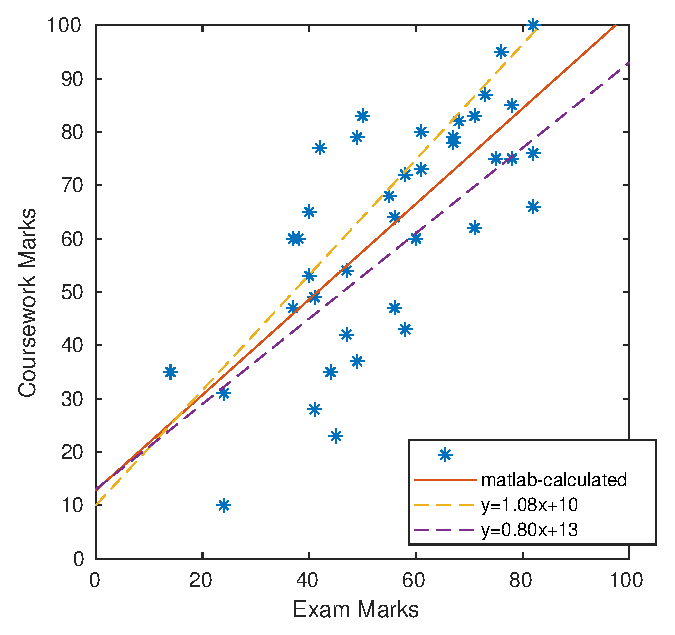
\includegraphics[scale=0.75, center]{./eps/topic1_c.eps}
	\caption{Coursework marks plotted against exam marks. }
	\label{fig:Topic1-c}
\end{figure}
By comparing the maximum and minimum fits, we find the uncertainties on slope ($\Delta a$) and y-intercept$(\Delta b)$ to be
\begin{equation}
\begin{split}
	&Y_{\max} = 1.08x + 10; \quad \quad Y_{\min} = 0.80x + 13 \\
	&\therefore \Delta a = \frac{1.08 - 0.80}{2} = 0.14; \quad \quad \Delta b = 1.5
\end{split}
\end{equation}
\lstinputlisting[caption={Topic 1. Question c. Note all code per topic belongs to same file}]{"./files/topic 1/c.m"}

\subsection{d}
The general trend is similar, but Matlab calculates a higher y-intercept $(12.7990)$ and a lower slope $(0.8950)$. This suggests that I overvalue the density of points towards the extremity of the graph, while the software appropriately looks at all points equally.
\subsection{e}
\begin{equation}
\begin{split}
	f(x) &= 0.8950x + 12.7990 \\
	f(60) &= 0.8950\cdot 60 + 12.7990 = 66.499
\end{split}
\end{equation}
Predicted grade would be 66.
\subsection{f}
We could present a more quantitative marker of reliability by measuring the correlation coefficient, but it can also be done qualitatively.
There is a general correlation between exam marks and coursework marks, but the scattering suggests this will be imperfect (have an R-coefficient less than 1).
From the data we have students with coursework marks around 60\% getting exam marks ranging from approximately 40\% to 80\%.
This is a really large spread that covers failing and getting first-class, so while the correlation is there, and it is accurate, it is not precise enough. 
\pagebreak